\begin{thm}{099}{\hosi 1}{高校入試}
 図のように、$\triangle{ABC}$の辺$AB$上に点$P$、辺$BC$上に点$Q, R$、辺$CA$上に点$S$を、四角形$PQRS$が長方形となるようにとる。黒く塗られた2つの三角形が相似になるとき、$\triangle{ABC}$の形状を全て答えよ。
 \begin{center}
  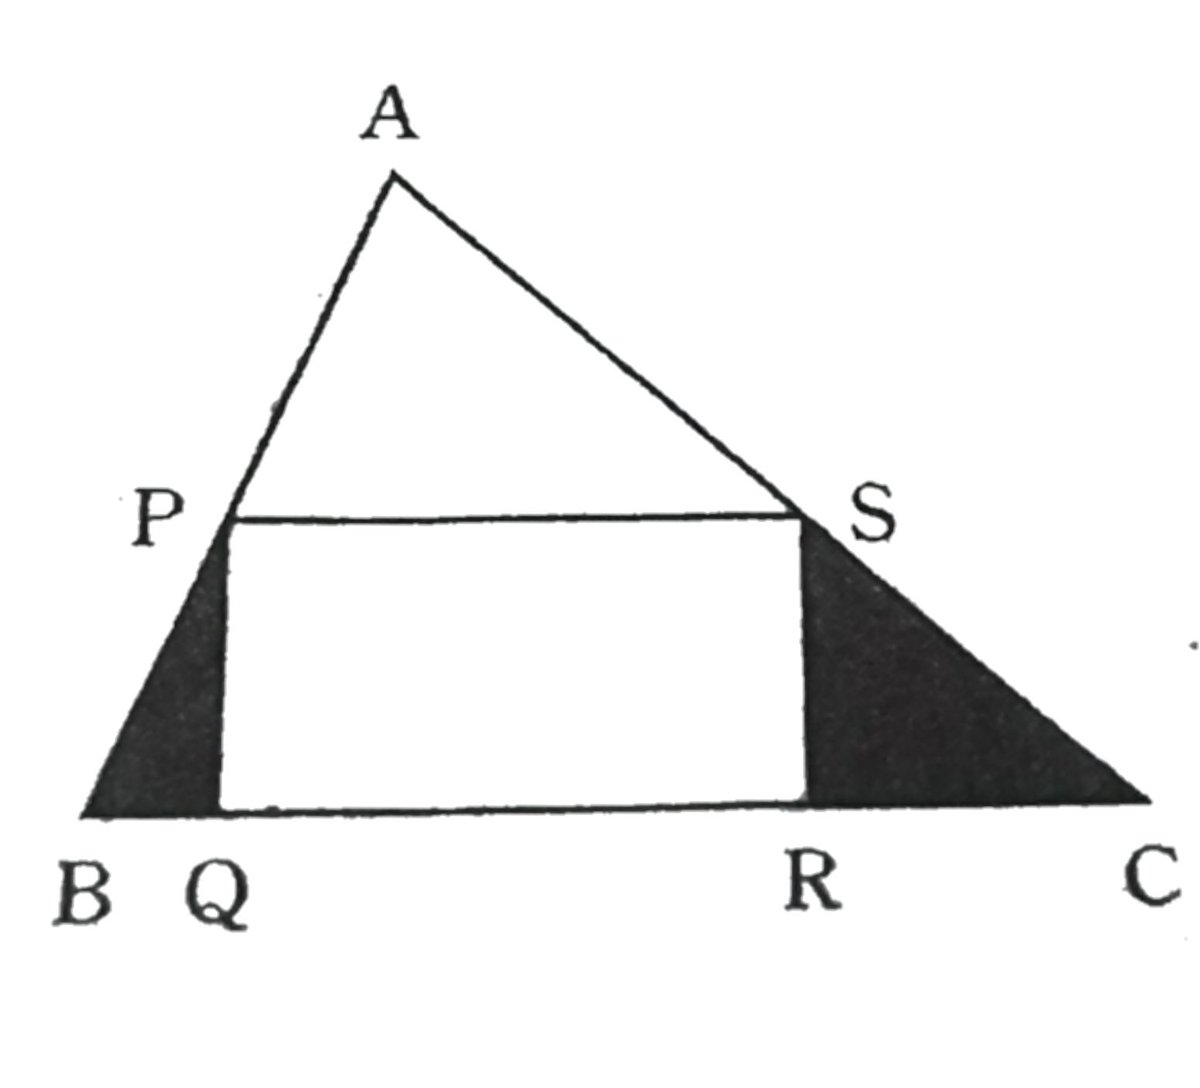
\includegraphics[bb=0 0 1200 1088,width=0.7\linewidth]{../problems/Q_099/Q_099.jpg}
 \end{center}
\end{thm}

ここに解答を記述。